%Datenstrukturen und Algorithmen
%	Was sind Algorithmen und Datenstrukturen
% 	Arten von Basis Datenstrukturen
%		Vector/Liste
%		Queue(Warteschlange)
%		Stack??
%		map und hash tabellen
%	besondere Datenstruktur - PCL Punktwolke
%	
%	Komplexität und Notation von Algorithmen
%	Arten von Basis Algorithmen
%		
% 		
%	besondere Algorithmen:
%		kd-tree
%		octree(vielleicht)
%		RANSAC
%		Segmentierung

\chapter{Theorie}
Im Kern dieser Arbeit steht eine Rechenaufgabe vor. Die positionellen Informationen über Objekte und Bauteile müssen sinnvoll verarbeitet werden, um die Lage und Form der geometrischen Merkmale des Objektes zu bestimmen. Bei der Entwicklung eines allgemeinen Verfahrens zur Erkennung der geometrischen Merkmale in Abschnitt~\ref{Methodik} werden Algorithmen und Datenstrukturen verwendet. 

\section{Datenstrukturen}

Datenstrukturen dienen der Organisation und Speicherung von Daten so, dass die Beziehung zwischen einzelnen Elemente auch aufbewahren wird. In einer Datenstruktur werden darüber hinaus auch Zugriffsmethoden für den Zugriff auf die gespeicherten Daten definiert sowie Angaben über Möglichkeiten zur Verarbeitung der Daten gemacht. Eine gute Datenstruktur setzt voraus, dass die Beziehung zwischen der Daten aufbewahren und gut definiert wird sowie die Verarbeitung der Daten leicht gemacht wird. Eine Datenstruktur soll auch bestimmte Operationen auf die Daten ermögliche, beispielsweise die Hinzufügung oder Entfernung von Datenpunkte, die Zusammenführung oder Sortierung der Daten sowie das Durchqueren der Datenstruktur und die Suche nach bestimmten Daten. In der Informatik gibt es bereits etablierte Datenstrukturen, die sich nach unterschiedlichen Einsatzzwecken richten und eine sehr breite Anwendung finden. Diese lassen sich nach Abbildung \ref{fig: datastructures} nach lineare und nichtlineare Datenstrukturen unterteilen. \autocite[1-2]{mohanty_data_2021}

\begin{figure}[h]
	\includegraphics[width=\textwidth]{Abbildungen/Datenstruktur_arten.png}
	\centering
	\caption{Die unterschiedlichen Arten von linearen und nichtlinearen Datenstrukturen nach \textcite[2]{mohanty_data_2021}}
	\label{fig: datastructures}
\end{figure}

\subsection{Lineare Datenstrukturen}
Eine lineare Datenstruktur ist eine Datenstruktur, bei der die Elemente in einer sequentiellen Reihenfolge angeordnet sind. Dies bedeutet, dass jedes Element genau einen Vorgänger und einen Nachfolger hat, außer dem ersten und letzten Element. Lineare Datenstrukturen können als tabellarische Liste oder als verkettete Liste implementiert werden. \autocite[314-315]{hoffmann_einfuhrung_2011}

Die Operationen, die auf einer linearen Datenstruktur ausgeführt werden können, sind in der Regel das Initialisieren der Datenstruktur als leere Menge, das Einfügen eines Elements in die Datenstruktur und das Entfernen eines Elements aus der Datenstruktur. Es ist auch möglich, andere Operationen auszuführen, die nicht unbedingt auf der Ordnungsbeziehung zwischen den Elementen basieren. Unter diesen Operationen zählen beispielsweise das Suchen nach einem Element oder das Ersetzen eines Elements in der Datenstruktur. \autocite[314-315]{hoffmann_einfuhrung_2011}

Die Implementierung einer linearen Datenstruktur kann je nach Anforderungen und verfügbaren Ressourcen variieren. Es ist jedoch wichtig sicherzustellen, dass die Datenstruktur korrekt implementiert ist und dass alle Operationen den Zustand der Datenstruktur ordnungsgemäß ändern. \autocite[314-315]{hoffmann_einfuhrung_2011}

Unter der linearen Datenstrukturen finden hauptsächlich drei Datenstrukturen eine breite Anwendung, nämlich Felder (Arrays), Schlangen (Queues) und Stapel (Stacks).

\subsubsection{Felder}

Das Feld ist einer der einfachsten linearen Datenstrukturen. Ein Feld besteht aus mehreren Daten des gleichen Formats oder Datentyps, die je nach Implementierung in aufeinanderfolgenden Speicherorten gespeichert werden. Diese werden sequenziell hintereinander angeordnet und zusammen gespeichert. Elemente eines Feldes dürfen eindimensional oder auch mehrdimensional gespeichert werden, wodurch diese Datenstruktur mit Matrizen oder Vektoren aus der Mathematik verglichen werden kann. Die Größe oder Dimension des Feldes wird immer vorgegeben und bleibt in der Regle statisch. Jedes Element eines Feldes besitzt einen sogenannten Index, welcher auf die Position des Elements in dem Feld deutet. Im Falle eines zwei Dimensionalen Feldes besitzt jedes Element der Datenstruktur zwei Indizes. In der regel deutet das erste Index auf die Zeile und das zweite Index auf die Spalte des Datenfeldes hin, allerdings kann dieser Regel von Implementierung zu Implementierung variieren. Felder dürfen eine beliebig Anzahl \textit{n} Dimensionen besitzen, allerdings steigt somit auch die Anzahl der Indizes aller Elemente. Datenfelder über vier Dimensionen können sogar räumlich nicht vorgestellt werden, jedoch macht es für einen Rechner kein Problem. Zugriffsoperationen auf Elemente sowie Operationen zur Einfügung und Entfernung dieser Elemente verwenden ihre Indizes, um den Eintrag an einer bestimmten Position des Feldes aufzurufen oder zu manipulieren. \autocite[35-36]{ollmert_datenstrukturen_2020}

Eine andere Variante der Felder ist die sogenannte lineare Liste. Diese Liste unterscheidet sich von Felder, indem sie dynamisch initialisiert werden darf. Im Gegensatz zu der statischen Größe oder Dimension eines Feldes, darf die Größe einer linearen Liste beliebig geändert werden. Während ein Feld mit maximale Größe \textit{n} und \textit{n} Elemente nicht um ein weiteres Element \textit{k} erweitert werden darf, kann eine lineare Liste der gleichen Größe mit den gleichen Anzahl an Elementen um das \textit{k-te} Element erweitert werden. Das Element darf auch an einer beliebigen Stelle der Liste eingefügt werden. Die Reihenfolge beziehungsweise die Positionen der anderen Elemente werden automatisch angepasst. Dies könnte auch dazu führen, dass ein Element Z, welches zum Zeitpunkt T1 vor der Einfügung eines neuen Elements einen bestimmten Index \textit{i} besaß, zu einem Zeitpunkt T2 nach der Einfügung nicht mehr an der gleichen Position zu finden ist. Das gleiche kann auch durch die Entfernung von Elementen an beliebigen Positionen geschehen. Die Positionen und somit die Indizes alle Elemente dürfen auch geändert werden, indem sie Beispielsweise nach einem Kriterium sortiert wurden. \autocite[40-42]{ollmert_datenstrukturen_2020}

Lineare Listen bieten viele ähnlichen Operationen wie die von Feldern an, um mit den eingespeicherten Elementen zu interagieren. Dazu gehört das Abrufen eines bestimmten Elements, das Einfügen eines neuen Elements zwischen zwei benachbarten Element (sowie Spezialfälle für das Hinzufügen eines neuen ersten oder letzten Elements), das Entfernen eines bestimmten Elements, das Bestimmen der aktuellen Länge der Liste anhand der Elementanzahl, die Suche nach einem Element mit einem bestimmten Wert, das Zusammenführen von zwei linearen Listen und das Aufteilen einer Liste in zwei Teillisten.\autocite[42-43]{ollmert_datenstrukturen_2020}


Verketteten linearen Listen sind eine bestimmte Art der Implementierung von linearen Listen. Eine solche Kette unterscheidet sich grundsätzlich nach ihrem Aufbau und Speicherverfahren von gewöhnlichen Listen und Feldern. Die Elemente einer verketteten linearen Liste werden nicht aufeinanderfolgend gespeichert. Stattdessen wird mit jedem Element dieser Liste auch ein Zeiger beigegeben, der entweder die Speicheradresse des nächsten Elements angibt oder auf das Ende der Liste hinweist. Der Anker ist ein besonderer Zeiger, der auf den Anfang der Liste deutet. Die Struktur und Operationen einer linearen Liste ist in Abbildung \ref{label} abgebildet. Bei der doppel-verketteten linearen Listen werden mit jedem Element nicht nur einen Zeiger zu dem nächsten Element beigegeben, sondern auch einen Zeiger zu dem vorigen Element. Bei dieser Art der verketteten Liste werden zwei Anker geliefert - der Vorwärtsanker für den Anfang und der Rückwärtsanker für das Ende der Liste. Die Verarbeitung mancher linearen Listen stellt eine Herausforderung dar, insbesondere wenn sie gleichzeitig durch mehrere Programme verarbeitet werden. In solchen Fällen könnte es beispielsweise dazu führen, dass ein Programm auf ein bestimmtes Element mittels seines Index zugreift, während ein anderes Programm ein Element davor hinzufügt oder entfernt. \autocite[43-44]{ollmert_datenstrukturen_2020}

\begin{figure}[t]
	\includegraphics[width=\textwidth]{Abbildungen/Verkettete_lineare_liste.png}
	\centering
	\caption{Die Struktur und Operationen einer linearen Liste. Die Großbuchstaben deuten auf die Elemente der Liste während die \textit{z}-Buchstaben die Zeiger repräsentieren. Die Kopfzelle steht in dieser Abbildung für den Anker.\autocite[611]{ernst_grundkurs_2020}}
\end{figure}

Für alle gängigen Implementierungen von linearen Listen ist die Implementierung einer sequentiellen Zugriffsfunktion, die das nächste Element in der Liste ausgehend von einem bestimmten Element bereitstellt, einfach. Die Implementierung einer direkten Zugriffsfunktion, die das \textit{i}-te Element in der Liste bereitstellt, ist zwar ebenfalls einfach, aber die benötigte Zeit hängt von der Position des Elements in der Liste ab und nimmt mit zunehmender Länge der Liste zu.\autocite[45]{ollmert_datenstrukturen_2020}

\subsubsection{Schlangen}
Schlangen sind besondere sequentielle Datenstrukturen, die Daten nur in einer bestimmten Reihenfolge speichern. Dadurch wird auch die Entnahme und Einfügung der Daten geregelt. Schlangen folgen das Prinzip nach \textit{First-In-First-Out} (FIFO), also werden die Elemente zur Verfügung gestellt, die zuerst zu der Datenstruktur hinzugefügt wurden. Elemente dürfen in der Regel nur am Ende der Schlange eingefügt und vom Anfang der Schlange entnommen werden. \autocite[371]{gumm_band_2016}

Das Prinzip nach \textit{FIFO} wird üblicherweise mittels verketteten linearen Listen ermöglicht. Der Anfang sowie das Ende der Schlange werden mittels Zeiger gekennzeichnet. Jedes Element, welches zu der Schlange hinzugefügt wird, erhält je nach Art der verketteten Liste einen Zeiger zu dem Element davor oder danach. Im Falle des ersten oder letzten Elements wird ihm ein besonderer Zeiger - der Nullzeiger - zugewiesen. Dieses deutet darauf hin, dass es keine weiteren Elemente zu finden sind. Der Zeiger \textit{anfang} deutet somit auf das vorderste und älteste Element der Schlange während der Zeiger \textit{ende} auf das hinterste und neuste Element deutet. Sobald der erste Eintrag der Schlange gelesen oder entnommen wird, wird der Zeiger \textit{anfang} inkrementiert, sodass es auf das nächste Element zeigt. Wenn ein neues Element zu der Schlange hinzugefügt wird, wird der Zeiger \textit{ende} inkrementiert, sodass es auf den letzten Eintrag der Schlange deutet. \autocite[48-49]{ollmert_datenstrukturen_2020} \autocite[371]{gumm_band_2016}

Schlangen bieten ähnliche Operationen wie Felder und Listen an. Im Gegensatz zu Listen oder Felder, wo Elemente mittels einem bestimmten Funktionsaufruf an beliebigen Positionen innerhalb der Datenstruktur platziert werden dürfen, dürfen Elemente aus einer Schlange nur am Ende eingefügt werden. Abhängig von der Implementierung wird eine Methode bereitgestellt, die das Einfügen eines Elements ermöglicht. Allgemein wird das Einfügen einer Datei in einer Schlange als \textit{enqueue} benannt.Felder und Liste ermöglichen mittels bestimmter Funktionen einen Zugriff auf beliebige Elemente innerhalb der Datenstruktur in einer beliebigen Reihenfolge. Bei Schlangen darf nur das erste Element aus der Datenstruktur entnommen werden, welches am längsten in der Datenstruktur enthalten wurde. Auch wird der Zugriff auf dieses Element abhängig von der Implementierung durch eine bestimmte Methode ermöglicht. Allgemein wird das entfernen oder auslesen eines Elements einer Schlange als \textit{dequeue} bezeichnet. Die Anzahl der Elemente \textit{count} in einer Schlange lässt sich bestimmen, indem die Differenz zwischen den Zeigern \textit{anfang} und \textit{ende} berechnet wird. In den meisten Implementierungen werden diese Schritte innerhalb einer Methode zur Bestimmung der Länge eingekapselt. Diese Operationen zusammen mit den zur Erstellung und Vernichtung von Schlangen sind die Einzigen Methoden, die für diese Datenstruktur in der Regel bereitgestellt werden. \autocite[71-72]{hubwieser_fundamente_2015} \autocite[371]{gumm_band_2016}

Die Ausführung der Prozeduren enqueue und dequeue erfordert bei einer Schlange einen konstanten Zeitaufwand, der unabhängig von der Anzahl der Elemente in der Datenstruktur ist. Die Suche nach einem Bestimmten Element in einer Schlange erfordert jedoch einen Zeitaufwand, der linear von der Anzahl der aktuellen Elemente in der Datenstruktur abhängt. Zur Überprüfung, ob ein bestimmtes Element in einer Schlange vorhanden ist, muss im Durchschnitt die Hälfte der Schlange durchsucht werden. \autocite[318]{hoffmann_einfuhrung_2011}

\begin{figure}[t]
	\includegraphics[width=\linewidth]{Abbildungen/Queue.png}
	\centering
	\caption{Eine Schlange mit den Operationen zur Einfügung und Entfernung von Elementen dargestellt \autocite[371]{gumm_band_2016}}
	\label{fig: queue}
\end{figure}

\subsubsection{Stapel}
Die Datenstruktur des Stapels, auch bekannt als Keller oder Stack, ist eine homogene, sequentielle Struktur, die nur das Einfügen und Lesen von Elementen am Anfang der Struktur erlaubt. Beim Lesen eines Elements wird dieses gleichzeitig entfernt, so dass das folgende Element an den Anfang rückt. Stapeln folgen das Prinzip nach \textit{First-In-Last-Out (FILO)} oder \textit{zuerst-rein-zuletzt-raus}. Die Anzahl der Speicherplätze des Stacks ist einseitig potenziell unbegrenzt, so dass der Stack dynamisch wachsen und schrumpfen kann. \autocite[614]{ernst_grundkurs_2020}

Stapel werden üblicherweise als verketteten linearen Listen implementiert, die nur in eine Richtung expandieren oder reduzieren dürfen. Somit erfolgt die Einfügung sowie die Entnahme von Elementen im Gegensatz zu Schlangen nur am einen Ende des Stapels. Bei der Einfügung jedes neuen Elements werden die Vorhandenen Elemente des Stapels zurückgeschoben und dem neuen Element wird einen Zeiger zum vorigen Element beigegeben. Im Falle des ersten Elements wird ihm ähnlich wie zuvor einen Nullzeiger zugewiesen, der auf dem Ende des Stapels hinweist. Elemente des Stapels dürfen nur in der umgekehrten Reihenfolge ausgelesen werden, in der Sie eingefügt wurden. Somit dürfte das allererste Element nur als allerletztes Element ausgelesen werden. \autocite[363]{gumm_band_2016}

Ähnlich wie Schlangen bieten Stapeln im Vergleich zu Felder und Listen nur begrenzte Funktionalitäten an. Elemente eines Stapels dürfen nicht an beliebigen Stellen zwischen vorhandenen Elementen des Stapels platziert werden, sondern nur am \textit{Kopf} des Stapels. Dieses wird durch die Operation \textit{push} ermöglicht, welches ein neues Element an der obersten Ebene platziert und den Zeiger für den Kopf nach oben nachrückt. Genau wie das Einspeichern darf das Auslesen eines Elementes nicht an einer beliebigen Stelle des Stapels erfolgen, sondern nur am Kopf des Stapels geschehen. Die Operation \textit{pop} ist dafür zuständig, das erste oder oberste Element des Stapels zu entfernen und für das Auslesen bereitzustellen. Gleichzeitig wird der Zeiger für den Kopf nach hinter gerückt, sodass es auf das vorige Element zeigt. Neben dieser Operationen werden auch für Stapeln zusätzliche Operationen bereitgestellt, die Stapeln erzeugen, vernichten oder seine Größe bestimmen. Wie diese Operationen definiert werden, hängt allerdings von der Implementierung ab. \autocite[614]{ernst_grundkurs_2020} \autocite[45-46]{ollmert_datenstrukturen_2020}

Im Prinzip funktioniert ein Stapel ähnlich zu einer Schlange, indem er das Auslesen oder Einfügen von Elementen nur an bestimmten Stellen erlaubt. \textit{Push} und \textit{pop} sind beide Operationen, die ähnlich wie \textit{enqueue} und \textit{dequeue} funktionieren und unabhängig von der Größe der Datenstruktur sind. Somit sollte der Zeitaufwand dieser Operationen auch konstant bleiben. Die Suche nach einem bestimmten Element in einem Stapel sollte ähnlich wie bei Schlangen direkt von der Anzahl der Elemente abhängen.

\begin{figure}[t]
	\includegraphics[width=\textwidth]{Abbildungen/Stack.png}
	\centering
	\caption{Ein Stapel mit den Operationen zur Einfügung und Entfernung von Elementen dargestellt \autocite[371]{gumm_band_2016}}
	\label{fig: stack}
\end{figure}

\subsection{Nichtlineare Datenstrukturen} \label{nicht_lineare_datenstrukturen}
Bei nichtlinearen Datenstrukturen werden Gegensatz zu linearen Datenstrukturen die einzelnen Elemente nicht in einer sequentiellen Reihenfolge zu einander stehen \autocite[321]{hoffmann_einfuhrung_2011}. 

Die Funktionsweise sowie die Operationen nichtlinearer Datenstrukturen lassen sich nicht verallgemeinern, sondern können von Implementierung zu Implementierung abweichen. Unter nichtlinearen Datenstrukturen finden hauptsächlich vier eine breite Anwendung, nämlich Bäume (Tree), Graphen (Graph), Tabellen (Tables) und Mengen (Sets). Im Rahmen dieser Arbeit werden nur Bäume und Graphen behandelt.

\subsubsection{Bäume}
Bäume stellen eine grundlegende Datenstruktur in der Informatik dar, die eine zweidimensionale Verallgemeinerung von Listen darstellen. Im Gegensatz zu Listen erlauben Bäume die Speicherung von Daten sowie die relevanten Beziehungen zwischen diesen Daten, wie beispielsweise Ordnungs- oder hierarchische Beziehungen. Daher sind Bäume besonders gut geeignet, um gesuchte Daten schnell wiederzufinden. Ein Baum besteht aus einer Menge von Knoten, die miteinander durch Kanten verbunden sind. Wenn eine Kante von Knoten A zu Knoten B führt, wird dies als A$\rightarrow$B notiert und A wird als Vater von B oder B als Kind von A bezeichnet. Ein Knoten ohne Kinder wird als Blatt bezeichnet, während alle anderen Knoten als innere Knoten bezeichnet werden. \autocite[389]{gumm_band_2016}

Ein Pfad von A nach B führt als Folge von Knoten und Pfeilen von A nach B, wobei die Knoten durch Pfeile verbunden sind. Dieser Pfad wird als A $\rightarrow$ X1 $\rightarrow$ X2 $\rightarrow$ $\cdot$ $\rightarrow$ B notiert, wobei die Länge des Pfades durch die Anzahl der Knoten bestimmt wird. Diese Anzahl kann 0 oder mehr betragen. Wenn es einen Pfad von A nach B gibt, so gilt B als Nachkomme von A, während A als Vorfahre von B bezeichnet wird. \autocite[389]{gumm_band_2016}

Ein Baum erfüllt verschiedene Axiome, die ihn von anderen Datenstrukturen unterscheiden. So gibt es genau einen Knoten, der als Wurzel bezeichnet wird und keinen Vater hat. Jeder andere Knoten hat genau einen Vater und ist ein Nachkomme der Wurzel. Zudem darf es keine zyklischen Pfade im Baum geben, da dies zu Widersprüchen führen würde. Ein weiteres Axiom besagt, dass es von der Wurzel zu jedem anderen Knoten genau einen Pfad gibt. Das bedeutet, dass jeder Knoten eindeutig bestimmt werden kann und es keine mehrdeutigen Wege durch den Baum gibt. Schließlich bilden die Nachkommen eines beliebigen Knotens K zusammen mit allen ererbten Kanten einen zusätzlichen Baum mit K als Wurzel. Dieser Baum wird als Unterbaum mit Wurzel K bezeichnet und erfüllt ebenfalls alle Axiome eines Baumes. Aufgrund dieser Eigenschaften sind Bäume besonders nützlich, hierarchische Strukturen abzubilden und Daten effizient abzuspeichern und wiederzufinden. \autocite[389]{gumm_band_2016}

Aufgrund der hierarchischen Aufbau und Form dieser Datenstruktur besitzt sie eine besondere Eigenschaft - die Tiefe. Die Tiefe wird anhand der Anzahl der Ebenen eines Baums bestimmt. Zur Bestimmung der Tiefe eines Baums wird der kürzeste Pfad zu der tiefsten Ebene des Baums verfolgt und dabei die Anzahl der Knoten aufgezählt. Diese Anzahl repräsentiert die Tiefe eines Baums. \autocite[390]{gumm_band_2016}

Eine exemplarische Abbildung eines Baums ist in Abbildung~\ref{fig: tree} zu sehen.

\begin{figure}[t]
	\includegraphics[width=\linewidth]{Abbildungen/Tree.png}
	\centering
	\caption{Ein Baum mit einer Tiefe von Fünf sowie die Darstellung der Beziehungen zwischen einzelner Knoten \autocite[390]{gumm_band_2016}}-
	\label{fig: tree}
\end{figure}

\textit{Binärer Baum} ist die Bezeichnung einer spezifischen Implementierung dieser Datenstruktur. Sie dient als einer der wichtigsten dynamischen Datenstrukturen. Binärer Bäume ermöglichen das Einfügen und Entfernen von Elementen zu der gleichen Geschwindigkeit wie Felder und einfachen linearen Listen. Darüber hinaus bieten Sie auch eine Möglichkeit an, die Suche nach bestimmten Elementen sowie das Durchsuchen innerhalb der Datenstruktur im Vergleich zu konventionellen sequentiellen Datenstrukturen zu beschleunigen. \autocite[617]{ernst_grundkurs_2020}

Alle Knoten eines binären Baums ausschließlich der Endknoten oder Blätter haben genau zwei Nachkomme oder Kinder. Darüber hinaus darf ein Vorfahre nicht zwei leere Nachkomme haben, sondern darf maximal nur ein Kind keinen Wert haben. Durch die Festlegung der ersten Bedingung wird es erzielt, dass jeder Vorfahre immer zu zwei Unterbäumen führt. Die zweite Bedingung verhindert das Aufblasen eines Baums, indem keine unnötigen leeren Unterbäume entstehen. Binäre Bäume dienen sind für die Aufgabe des Suchens besonders geeignet. Sie dienen der effizienten binären (Ja/Nein) Auswertung von Aussagen. Bäume für diesen Zweck werden oft als binäre Suchbäume bezeichnet. Ein binärer Suchbaum ist genau so wie ein allgemeiner binärer Baum aufgebaut, indem jeder Knotenpunkt einen linken und rechten Unterbaum besitzt. Jeder Knoten enthält einen Schlüsselwert, der ihm zugeordnet ist. Eine wichtige Eigenschaft von binären Suchbäumen ist, dass der Schlüsselwert eines jeden Knotens größer ist als alle Schlüsselwerte im linken Unterbaum des Knotens und kleiner als alle Schlüsselwerte im rechten Unterbaum des Knotens. \autocite[94-95]{ollmert_datenstrukturen_2020}

Um nach einem Element in einem binären Suchbaum zu suchen, wird zuerst der Wert der Wurzel überprüft. Falls dieser nicht dem Element beträgt werden die nächsten Nachkomme der Wurzel überprüft. Hierbei werden allerdings nicht beide Kinder der Wurzel mit dem Element vergleicht, sondern wird der Wert des Elements zuerst mit dem der Wurzel verglichen. Sei das Elements kleiner als die Wurzel, wird nur das linke Kind beziehungsweise Unterbaum weiter untersucht. Sei das Element stattdessen größer, wird der rechter Unterbaum untersucht. Dieses wird rekursiv wiederholt, bis ein Konten mit dem Wert des Elements gefunden wird. Bei der meisten Implementierung der Suchfunktion erfolgt das allerdings iterativ und nicht rekursiv. Dieser Vergleich wird solange wiederholt, bis das Element gefunden wird. \autocite[139-140]{knebl_algorithmen_2021}

Um ein Element in dem Suchbaum einzufügen erfolgen die folgenden Schritte. Mittels der Suchfunktion wird zuerst überprüft, ob das Element bereits in dem Suchbaum vorhanden ist. Im Falle des Vorhandenseins wird die Funktion aufgehalten. Anderweitig wird der Wert des Blattes aufgerufen, wo die Suchfunktion aufgehört hat. Dank der Funktionsweise eines binären Baums wird der Wert des neuen Elements ähnlich Groß wie der des Blattes sein. Das Blatt wird zu einer Wurzel eines Unterbaums gewandelt. Falls der Wert des neuen Elements kleiner als der des Blattes ist, wird es links im Unterbaum gespeichert. Ansonsten wird es rechts im Unterbaum gespeichert. \autocite[140]{knebl_algorithmen_2021}

Beim Löschen eines Elements wird der gleiche erst Schritt wie beim Einfügen verwendet. Mittels der Suchfunktion wird sichergestellt, dass das Element in dem Baum vorhanden ist. Falls das Element in einem Blatt gespeichert ist, erfolgt die Löschung sehr einfach, indem das Blatt vom Baum entfernt wird und der Vorfahre aktualisiert wird, somit es nicht auf das leere Blatt zeigt. Die Entfernung des Elements erfolgt auch relativ simpel im Falle, dass das Knoten \textit{v} des Elements nur einen Nachkomme hat. In diesem Fall wird der Vorfahre des Knotens \textit{v} geändert, sodass es auf das Nachkomme des Knotens \textit{v} zeigt. Danach wird das Knoten \textit{v} gelöscht. Problematischer wird die Löschung wenn das Knoten \textit{v} des Elements zwei Nachkomme besitzt. Hierfür wird in dem linken Unterbaum von \textit{v} möglichst tief nach dem größten Wert \textit{$\overline{e}$} gesucht. Dieser Wert wird möglichst tief und rechts liegen. Dieser Wert wird sowohl größer als andere Werte im linken Unterbaum sein als auch kleiner als dem Element. Dieser Wert darf maximal einen linken Nachkomme besitzen. Sobald \textit{$\overline{e}$} bestimmt wird, wird dieser Wert anstelle des Elements in \textit{v} eingefügt. Der linke Nachkomme von \textit{$\overline{e}$} wird somit der rechte Nachkomme von dem vorigen Vorfahre von \textit{$\overline{e}$}. Somit wird es erzielt, das Element aus dem Baum zu löschen und die binäre Eigenschaft des Suchbaums aufrechterhaltenen. Die Abbildung~\ref{fig: tree_delete} visualisiert dieses Verfahrens. \autocite[140-141]{knebl_algorithmen_2021}

\begin{figure}[!b]
	\includegraphics[width=\linewidth]{Abbildungen/tree_delete.png}
	\centering
	\caption{Eine Veranschaulichung des Löschvorgangs in einem binären Suchbaum \autocite[140]{knebl_algorithmen_2021}}
	\label{fig: tree_delete}
\end{figure}

Neben dem Suchbaum gibt es auch andere Varianten des binären Baums, die unterschiedlichen Eigenschaften aufweisen und besondere Funktionalitäten anbieten. Unter diesen sind B-Bäume und AVL-Bäume einer der gängigsten Varianten, die häufig eine Anwendung finden. B-Bäume eignen sich insbesondere für das Speichern und effiziente Verwalten von sehr großen Datenmengen während AVL-Bäume, aufgrund ihrer bilanzierten Struktur, Suchfunktionen besonders schnell ausführen können. Die genauere Untersuchung der Struktur und Funktionsweise dieser Varianten liegt allerdings außerhalb des Umfangs dieser Arbeit \autocite[407-412]{gumm_band_2016}.

\subsubsection{Graphen}
Diese Datenstruktur findet ihre Herkunft in dem Teilgebiet des diskreten Mathematik in der sogenannten Graphentheorie. Graphen werden anschaulich als eine Menge von Knoten dargestellt, die durch Kanten miteinander verbunden sind. Sie umfassen eine sehr allgemeine Klasse von Datenstrukturen, welche andere Strukturen wie Bäume und lineare Listen als Teilmenge enthalten. In der Praxis haben Graphen eine große Bedeutung, da sich sehr viele statische und dynamische Strukturen der realen Welt darauf abbilden lassen. Straßenverbindungen, Kommunikations- und Rechnernetze, Flussdiagramme, Automaten, elektronische Schaltpläne sind Beispiele dafür. \autocite[215]{knebl_algorithmen_2021} \autocite[654]{ernst_grundkurs_2020}

Durch die Verbindung von Knoten mit Kanten in einem Graph soll die Relationen zwischen den Datenelemente darstellen. Die Kanten verbinden jeweils zwei Knoten miteinander und können ungerichtet oder gerichtet sein. Ungerichtete Kanten stellen eine Verbindung zwischen zwei Knoten dar, ohne eine bestimmte Richtung anzugeben. Gerichtete Kanten hingegen haben eine bestimmte Richtung und stellen eine Verbindung von einem Knoten zu einem anderen dar. \autocite[221-222]{knebl_algorithmen_2021}

Für die Suche nach einem Datenelement innerhalb des Graphen müssen Graphen durchquert werden. Die Breitensuche und Tiefensuche sind zwei etablierte Verfahren, die dazu dienen. Bei der Breitensuche (Breadth-First Search, BFS) wird der Graph schichtenweise durchsucht. Zu Beginn wird ein Startknoten gewählt und seine direkten verbunden benachbarten Knoten (Nachbarn) werden besucht. Anschließend werden die Nachbarn der Nachbarn sequentiell weiterhin besucht, bis alle Knoten besucht wurden oder ein bestimmter Zielknoten gefunden wurde. Das besondere an diesem Verfahren ist, dass ein Knoten nur dann besucht, wenn er noch nicht besucht wurde. Diese Tatsache verleiht diesem Verfahren seine besonders hohe Geschwindigkeit bei einem Suchvorgang. Um zu verhindern, dass der Algorithmus in einer Endlosschleife landet, werden die besuchten Knoten in einem Stapel gespeichert. \autocite[227-228]{knebl_algorithmen_2021} \autocite[666]{ernst_grundkurs_2020}

Bei der Tiefensuche (Depth-First Search, DFS) wird der Graph hingegen rekursiv durchsucht. Auch hier wird ein Startknoten gewählt, dessen erster direkter Nachbar besucht wird. Nachdem der erster Nachbar besucht wurde, wird dessen direkter Nachbarn wieder besucht. So werden sequentiell die Nachbarknoten von Nachbarknoten durchquert, bis ein Endknoten erreicht wird. Danach wird der vorherige Knoten wieder ausgewählt und sein nächster Nachbar besucht. Das Verfahren wird solange fortgesetzt, bis alle Knoten besucht wurden. Auch hier werden die besuchten Knoten markiert, um zu verhindern, dass der Algorithmus bereits besuchten Knoten wieder besucht und in einer Endlosschleife landet. Zur Aufspeicherung der bereits besuchten Knoten wird an der Stelle eine Schlange verwendet. \autocite[231-232]{knebl_algorithmen_2021} \autocite[666]{ernst_grundkurs_2020}

\begin{figure}[t]
	\centering
	\begin{subfigure}[h]{0.49\textwidth}
		\includegraphics[width=\linewidth]{Abbildungen/Breitensuche.png}
		\centering
		\caption{Eine Visualisierung der Breitensuche nach \textcite[228]{knebl_algorithmen_2021}}
		\label{fig: breitensuche}
	\end{subfigure}
	\hfill
	\begin{subfigure}[h]{0.49\textwidth}
		\includegraphics[width=\linewidth]{Abbildungen/Tiefensuche.png}
		\centering
		\caption{Eine Visualisierung der Tiefensuche nach \textcite[232]{knebl_algorithmen_2021}}
		\label{fig: tiefensuche}
	\end{subfigure}
	\caption{Eine Visualisierung beider Suchverfahren für Graphen}
	\label{fig: graph_search_functions}
\end{figure}

Wie bereits ertönt, Graphen eignen sich zur Speicherung von statischen und dynamischen Strukturen der reellen Welt. Mittels Algorithmen wie Dijkstras Algorithmus können gewichtete Graphen kostengünstig durchquert werden. Die Kanten eines gewichteten Graphen erhalten auf Basis der Kosten (Beispielsweise Zeit oder Streckenlänge) zur Durchquerung über der Kante eine Gewichtung. Die kürzesten oder schnellsten Pfade zwischen Knoten können somit gefunden werden. Andere Algorithmen wie Prims Algorithmus dienen der Ermittelung des minimalen Spannbaums eines Graphen. Ein Spannbaum könnte als ein Teilgraph \textit{T} definiert werden, der alle Knoten eines Graphen \textit{G} enthält, allerdings weniger Kanten. Trotzdem sind alle Knoten eines Spannbaums vollständig vernetzt. Ein minimaler Spannbaum ist ein Teilgraph eines gewichteten Graphen, dessen Summe der Gewichte weniger als alle andere möglichen Spannbäume ist. Prims Algorithmus lässt sich besonders gut für Routing-Probleme in lokalen Rechnernetze verwenden. \autocite[277-282]{hubwieser_fundamente_2015}

\subsection{Datenstruktur zur Speicherung mehrdimensionalen Daten}

Ein k-dimensionaler Baum , der auch als kd-Baum bekannt ist, ist eine geometrische Datenstruktur, die dazu dient, mehrdimensionale Punkte in einem verbesserten binären Suchbaum zu organisieren. Dabei werden raumbezogene Suchanfragen bearbeitet, indem über Dimensionen alternativ gesucht wird. \autocite[92]{saha_advanced_2019} \autocite{bentley_fast_1978}

Der KD-Baum ist die gängigste räumliche Datenstruktur für die Durchführung von Bereichs- und nächsten Nachbarschafts-Suchanfragen. In jeder Ebene des Baums werden alle Kinder entlang einer bestimmten Dimension partitioniert. Danach wird in der nächsten Ebene diese Dimension über eine Hyperebene gedreht, die senkrecht zur Betrachtungsachse steht. Zu Beginn des Baums werden alle Punkte basierend auf der ersten Koordinate des Wurzelknotens partitioniert, so dass alle Punkte des rechten Teilbaums größere erste Koordinaten haben als die Wurzel. Im Umkehrschluss ist der Wert der ersten Dimension oder Koordinate aller Punkte im linken Teilbaum kleiner. Jede Ebene des Baums partitioniert den Suchraum basierend auf der nächsten Dimension und kehrt periodisch zur ersten Dimension zurück, wenn die letzte abgeschlossen ist. Der effizienteste Weg zur Erstellung eines statischen KD-Baums besteht darin, eine Partitionierungsmethode zu verwenden, die den Medianwert der Raumpunkte verwendet. Dabei bewegen sich Daten mit kleineren eindimensionalen Werten nach links und Daten mit größeren Werten nach rechts. Dieser Vorgang wird dann rekursiv auf beide Teilbäume wiederholt, bis nur noch ein Element übrig bleibt. Dieses Element wird als Blatt des Baumes gespeichert. \autocite[92]{saha_advanced_2019}

Die Erstellung eines statischen kd-Baums für \textit{n} Raumpunkte in \textit{d} Dimensionen erfolgt nach den folgenden Schritten. Zuerst wird der Median der Randpunkte ermittelt und in dem Wurzel des Baums platziert. Danach wird die erste Dimension der \textit{d} Dimensionen verwendet, um eine Hyperebene zu erstellen. Falls \textit{d} gleich zwei ist, wird eine Linie erstellt. Falls \textit{d} drei beträgt, wird eine zweidimensionale Ebene erstellt. Diese Hyperebene teilt die Raumpunkte gleichmäßig auf. Alle Punkte mit einer kleineren ersten Dimension befinden sich somit links zur Hyperebene und Punkte mir einer größeren ersten Dimensionen an der rechten Seite. Die linken und rechten Seiten der Hyperebenen werden in Teilbäume aufgespeichert. Danach werden die Medianwerte der Punkte der jeweiligen Teilbäume ermittelt und auf Basis der nächsten Dimension wieder mittels einer Hyperebene aufgeteilt. Diese Schritte werden rekursive für Teilbäume wiederholt, wobei die Dimension zur Erstellung der Hyperebene für jede sukzessive Ebene zyklisch gewechselt wird. Bis zum Ende dieses Zyklus werden alle Punkte so partitioniert, dass am Ende des Baums nur Blätter vorhanden sind. Abbildung \ref{fig: kd-tree_creation} bildet einen kd-Baum ab und visualisiert seine Erstellung. \autocite[93-94]{saha_advanced_2019} 

% Die Erstellung eines kd-Baums erfolgt mit einer Komplexität von $O(n\log n)$, wobei \textit{n} die Anzahl der Punkte beträgt.

\begin{figure}[!b]
	\includegraphics[width=\textwidth]{Abbildungen/2d_kd-tree.png}
	\centering
	\caption{Visualisierung eines zweidimensionalen kd-Baums sowie des Prozesses zur Erstellung dieses Baums \autocite[60]{garcica-garcia_alberto_towards_2015}}
	\label{fig: kd-tree_creation}
\end{figure}

Da das kd-Baum einen binären Baum als die grundlegende Datenstruktur verwendet, können alle Operationen eines allgemeinen binären Baums auf kd-Bäume angewendet werden. Mittels einer Suchoperation wird die Suche nach einem bestimmten Raumpunkt innerhalb der Baumstruktur ermöglicht. Bei der Suche nach einem bestimmten Punkt \textit{p} wird die seine erste Dimension mit der des Wurzels verglichen. Falls der Punkt kleiner als der Median ist, wird im linken Teilbaum weitergesucht. Ansonsten gelangt das Verfahren zum rechten Teilbaum. Danach wird die zweite Dimension von \textit{p} mit der zweiten Dimension der Wurzel des Teilbaums verglichen, um den nächsten Nachkomme zu bestimmen, wohin die Suche gelangen wird. Diese Schritte werden rekursiv wiederholt, bis der Punkt \textit{p} gefunden wird. Das Einfügen sowie die Entfernung von Elementen aus einem kd-Baum erfolgt analog zu den allgemeinen Verfahren für binären Bäume aus Abschnitt~\ref{nicht_lineare_datenstrukturen}. \autocite[94]{saha_advanced_2019}

Eine besondere Eigenschaft des kd-Baums ist die Möglichkeit schnell und effizient nach einer bestimmten Anzahl von Nachbarpunkte eines Raumpunktes zu suchen. Dies erfolgt nach zwei Verfahren - die Bereichssuche und die Suche der nächsten Nachbarschaft. Gewöhnlich wird die Bereichssuche von kd-Bäume eingesetzt, um alle Punkte innerhalb eines vorbestimmten sphärischen Radius \textit{R} zu finden. Hierfür wird ein Stapel verwendet. Zuerst wird der Mittelpunkt \textit{m} des sphärischen Bereiches festgelegt, der häufig ein bereits vorhandener Raumpunkt des kd-Baums ist. Die Suchfunktion des Baums beginnt dabei bei dem Wurzel quert abhängig von der Dimensionen von \textit{m} durch die Unterbäume durch. Bei dem Suchverlauf werden alle durchquerten Knoten sowie deren Nachkomme zu dem Stapel eingefügt. Wenn ein Blatt des Baums erreicht wird, werden die eingespeicherten Punkte in dem Stapel der Reihe nach ausgelesen und die Abstände zwischen dem Punkt und \textit{m} bestimmt. Liegt der Abstand eindeutig unter dem Wert \textit{R}, wird der Punkt akzeptiert und abgespeichert. Befindet sich ein Punkt auf den Umfang der Sphäre, werden die Abstände seiner Kinder zum \textit{m} bestimmt. Dabei werden alle Kinder ausgeschlossen, die außerhalb des Radius \textit{R} liegen. Abhängig von der Implementierung ergibt sich auch die Möglichkeit, die Suche auf die ersten \textit{k} Punkte zu beschränken. \autocite[95]{saha_advanced_2019}

Bei einer Suche nach dem nächsten Nachbar in einem kd-Baum wird ähnlich wie bei einer Bereichssuche vorgegangen, nur dass der Radius \textit{R} als aktuelles Minimum und Ablehnungskriterium anstatt als akzeptierte Bedingung behandelt wird. Die Suche nach dem nächsten Nachbar wird verwendet, um den nächsten Punkt in unmittelbarer Nähe zu einem bestimmten Punkt \textit{p} zu finden. Auch in dieser Suche wird ein Stapel verwendet. Mit der Suchfunktion wird ein binärer Vergleich zwischen dem Wert von \textit{p} und einen Knoten (am Anfang die Wurzel) ausgeführt und abhängig davon durch den linken oder rechten Teilbaum durchquert. Dabei werden alle besuchten Knoten auf dem Suchpfad und deren Kinder zu dem Stack so lange eingefügt, bis ein Blatt des Baums erreicht wird. Die Entfernung dieses Blatts zu dem Abfragepunkt \textit{p} wird ermittelt und als aktuelles Minimum \textit{R} betrachtet. Danach werden die Punkte aus dem Stapel sukzessiv ausgelesen und der Abstand zwischen ihnen und \textit{p} berechnet. Sei dieser Abstand kleiner als \textit{R}, wird der Wert von \textit{R} aktualisiert, um den neuen kürzesten Abstand zu entsprechen. Wenn der Stapel leer ist, wird der Punkt mit dem kürzesten Abstand zu \textit{p} als der nächste Nachbar zurückgegeben. Abhängig von der Implementierung wird es auch ermöglicht, die ersten \textit{k} nächsten Nachbarn von \textit{p} zu bestimmen. \autocite[96]{saha_advanced_2019}

Da kd-Bäume mit sehr hohen Datenmengen sowie mit einer hohen Dimensionalität umgehen müssen, ist es von hohem Wert, wenn die Laufzeiten der einzelnen Operationen eines kd-Bäums geschätzt werden könnten. Hierfür wird die O-Notation verwendet, die in Abschnitt~\ref{o-notation} detaillierter behandelt wird. Die Zeitkomplexität des Initialisierungs- und Erstellungsverfahrens beträgt $O(n\log n)$. Die Suchfunktionen für einen bestimmten Punkt in dem Baum hat im Gegensatz eine niedrigere Zeitkomplexität von $O(\log n)$. Das Einfügen und Entfernen eines Elements sowie die Bereichssuche und Suche nach nächsten Nachbarn hat normalerweise auch die gleiche Zeitkomplexität. Allerdings sei es mit einer sehr hohen Anzahl an Dimensionen sowie einem unsymmetrischen  kd-Baum möglich, dass die Zeitkomplexität der Bereichssuche sowie der Suche des nächsten Nachbars auf $O(k \cdot n^{1-\frac{1}{k}})$ steigt. \autocite[104-105]{bentley_fast_1978} \autocite[94-96]{saha_advanced_2019}

Es lässt sich feststellen, dass ein wichtiges Element aller Datenstrukturen die Verfahren oder Algorithmen sind, die zur Interaktion mit oder zur Manipulierung von der Datenstruktur verwendet werden.

\section{Algorithmen}
Ein Algorithmus ist ein Verfahren, welches zur Bestimmung einer oder mehreren Lösungen eines bestimmten Rechenproblems verwendet wird \autocite[1]{knebl_algorithmen_2021}. In einem Algorithmus wird ein Lösungsansatz möglichst präzise ausformuliert, indem kleine, isolierte und klar definierte Verarbeitungsschritte definiert werden. Auch ein simples Verfahren zur Summierung zwei Zahlen lässt sich als ein Algorithmus nennen. \autocite[9-10]{hubwieser_fundamente_2015}

Gewisse strukturelle Gemeinsamkeiten sind bei allen Algorithmen vorhanden, auch wenn sie in verschiedenen Darstellungsarten unterschiedlich beschrieben werden können. Algorithmen beschreiben Berechnungen durch die Verwendung von elementaren Verarbeitungsschritten sowie Sequenzen, bedingten Verarbeitungsschritten und Wiederholungen von elementaren Verarbeitungsschritten. Diese Bausteine werden auch als Strukturelemente von Algorithmen bezeichnet. \autocite[12]{hubwieser_fundamente_2015}

Es gibt simple, nicht-zusammengesetzte  Verarbeitungsschritte, die zwingend ausgeführt werden müssen. Zusätzlich zu diesen elementaren Verarbeitungsschritten sind noch drei Arten von zusammengesetzten Verarbeitungsschritten erforderlich, um Abläufe zu beschreiben: Sequenzen, bedingte Verarbeitungsschritte und Wiederholungen. \autocite[12]{hubwieser_fundamente_2015}

Elementare Verarbeitungsschritte können zu Sequenzen zusammengefasst werden, um hintereinander auszuführende Schritte darzustellen. Jeder Schritt übernimmt dabei das Ergebnis seines Vorgängers. Zur Trennung der einzelnen Komponenten einer Sequenz wird ein festes Trennzeichen festgelegt, wie beispielsweise ein Strichpunkt oder ein Zeilenwechsel. In manchen Programmiersprachen können Sequenzen auch mit Begrenzungssymbolen (beispielsweise geschweiften Klammern) zu einem Block zusammengefasst werden.\autocite[12]{hubwieser_fundamente_2015}

Bei einigen Verarbeitungsschritten ist es notwendig, dass sie nur unter bestimmten Bedingungen ausgeführt werden. In solchen Fällen kann es auch erforderlich sein, alternative Verarbeitungswege festzulegen, die ausgeführt werden, wenn die Bedingung nicht erfüllt ist. Diese Art von Verarbeitungsschritten wird als bedingte Verarbeitungsschritte bezeichnet. Bei bedingten Verarbeitungsschritten dürfen sowohl elementare als auch zusammengesetzte Verarbeitungsschritte ausgeführt werden. \autocite[12-13]{hubwieser_fundamente_2015}

Es ist häufig notwendig, dass Sequenzen von Verarbeitungsschritten mehrfach ausgeführt werden. Dabei werden bestimmte Bedingungen definiert, um die Anzahl der Wiederholungen zu regeln. Es ist möglich, sowohl elementare Verarbeitungsschritte als auch zusammengesetzte Verarbeitungsschritte zu wiederholen. Dabei gibt es einen Unterschied zwischen zwei Arten von Wiederholungen: solchen mit einer vorgegebenen Anzahl von Wiederholungen und solchen mit einer Bedingung, die zu Beginn oder am Ende der Wiederholung geprüft wird. Die letztere Art ist sicherer, während die erstere flexibler ist und eine größere Vielfalt von Funktionen ermöglicht. \autocite[13-14]{hubwieser_fundamente_2015}

\subsection{Komplexitätsmaße von Algorithmen} \label{o-notation}
Die Asymptotische Analyse ist eine Disziplin der Informatik, die sich mit der Bestimmung des Aufwands von Algorithmen zur Lösung von Problemen beschäftigt. Dabei werden insbesondere die Zeitkomplexität und die Speicherkomplexität betrachtet. In diesem Zusammenhang soll im Folgenden nur auf die zeitliche Komplexität eingegangen werden, da der verfügbare Speicherplatz in der heutigen Zeit in der Regel ausreichend ist und zudem immer preisgünstiger wird. Dennoch lassen sich die angewandten Analyse-Techniken auch auf die Untersuchung des Speicherbedarfs übertragen. \autocite[201]{hubwieser_fundamente_2015}

Eine Möglichkeit, die Laufzeit eines Algorithmus zu bestimmen, wäre die Durchführung von Tests mit verschiedenen Eingabegrößen. Dieses Vorgehen ist jedoch häufig unpraktikabel, da manche Algorithmen für größere Eingaben so lange laufen, dass eine Messung nicht durchführbar ist. Zudem würde die zum Testen verwendete Hardware das Ergebnis beeinflussen, was für eine aussagekräftige Effizienzbewertung unerwünscht ist.\autocite[201]{hubwieser_fundamente_2015}

Aus diesen Gründen werden in der Asymptotischen Analyse Techniken verwendet, die unabhängig von der Hardware sind und auf mathematischen Überlegungen basieren. Dabei wird der Aufwand eines Algorithmus in Abhängigkeit von der Größe der Eingabe analysiert. Das Ergebnis dieser Analyse sind sogenannte Laufzeitfunktionen, die das Wachstum des Algorithmus in Bezug auf die Größe der Eingabe beschreiben. Durch die Verwendung von Notationsmethoden wie der O-Notation können die Laufzeitfunktionen kompakt und übersichtlich dargestellt werden. Dies ermöglicht es, Algorithmen auf ihre Effizienz hin zu vergleichen und geeignete Algorithmen für spezifische Problemstellungen auszuwählen.\autocite[201-203]{hubwieser_fundamente_2015}

Es hat sich bei der asymptotischen Analyse etabliert, drei verschiedenen Maße für die Zeitkomplexität zu verwenden. Bei dem besten Fall (englisch: best case) \textit{T\textsubscript{best}} wird der Fall des Algorithmus betrachtet, der am schnellsten gelaufen ist. Bei dem schlimmsten Fall (englisch: worst case) \textit{T\textsubscript{worst}} wird die langsamste Berechnungsdauer eines Algorithmus ins Betracht gezogen. Um die durchschnittliche Dauer der Berechnung anzugeben, wird der Durchschnittsfall (englisch: average case) \textit{T\textsubscript{avg}} verwendet. Der beste Fall eines Algorithmus ist in den meisten Fällen irrelevant, da Programme meistens gegen dem schlimmsten Fall gesichert werden müssen. Hier sind die Maße \textit{T\textsubscript{worst}} oder \textit{T\textsubscript{avg}} von höherer Bedeutung. \autocite[202]{hubwieser_fundamente_2015}

Die Angabe der Zeitkomplexität mittels Einheiten der Zeit wie Sekunden lässt das Treffen einer allgemeinen Aussage über die Effizienz des Algorithmus nicht zu. Vielmehr hilft die Modellierung der Zeitkomplexität als eine Funktion der Eingabegröße, da sie eine Abstrahierung der Effizienz ohne den Einfluss von Faktoren wie Hardware ermöglicht. Zur Angabe der Zeitkomplexität wird am gängigsten das Landau-Symbol oder die \textit{O-Notation} verwendet. Das Wachstumsverhalten der benötigten Berechnungsdauer eines Algorithmus wird gegen eine unendliche große Eingabegröße aufgezeichnet, indem die Eingabegröße möglichst hohe Werte annimmt. Zeigt die Zeitkomplexität eine polynomialen Trend, wird zur Darstellung der Zeitkomplexität der höchste Grad der Funktion verwendet. Konstante werden bei der O-Notation auch nie berücksichtigt. Der Verlauf der Zeitkomplexität gegen steigender Eingabegröße kann auch einen logarithmischen Trend aufweisen. Die Tabelle \ref{table: o-notation} fasst alle gängige Komplexitätsgrade, die häufig verwendet werden. \autocite[203]{hubwieser_fundamente_2015}

\begin{table}[t]
	\centering
	\begin{tabular}{{l}{r}}
		\hline
		\textbf{Notation} & \textbf{Sprechweise} \\
		\hline
		$O(1)$ & konstant \\
		$O(\log (n))$ & logarithmisch \\
		$O(n)$ & linear \\
		$O(n\log (n))$ & log-linear \\
		$O(n^2)$ & quadratisch \\
		$O(n^k, k > 2)$ & polynomial \\
		$O(k^n), k \geq 2$ & exponentiell \\
		\hline
	\end{tabular}
	\caption{Die gängigen Varianten der O-Notation, sortiert nach steigender Zeitkomplexität \autocite[205]{hubwieser_fundamente_2015}}.
	\label{table: o-notation}
\end{table}

\begin{figure}[!b]
	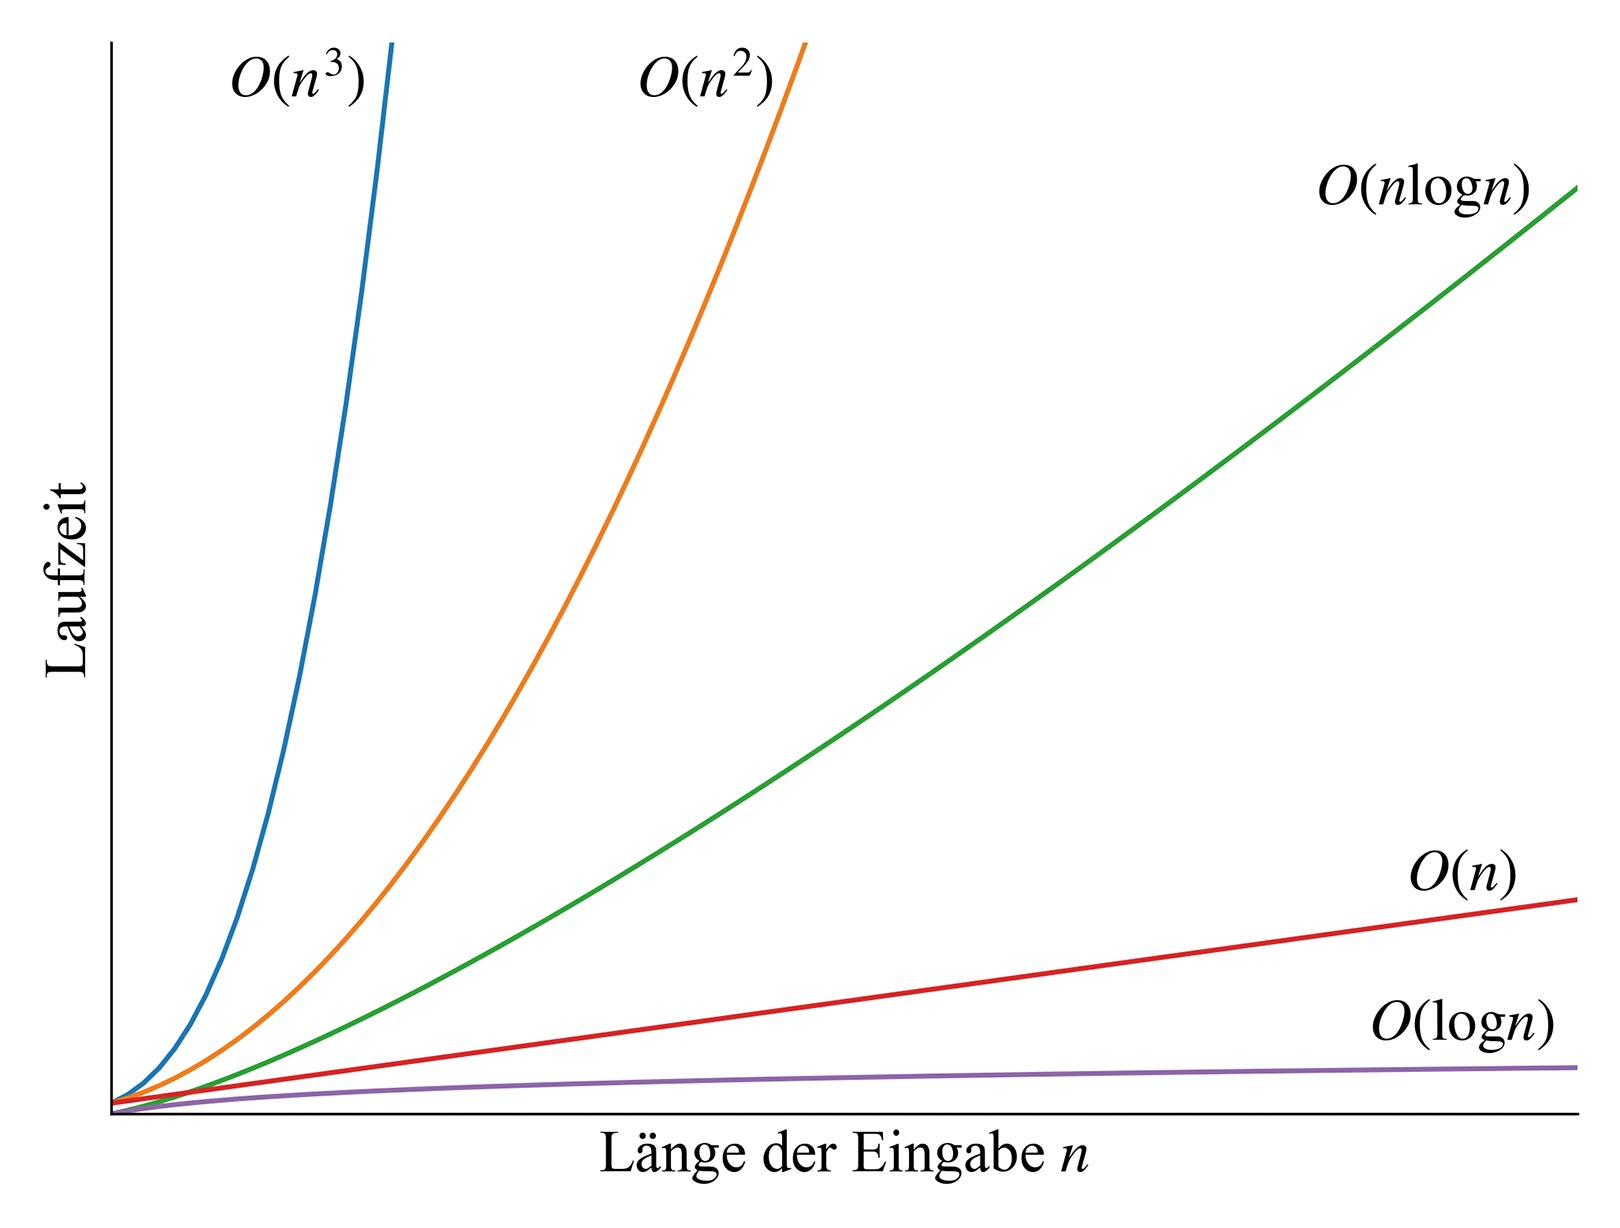
\includegraphics[scale=0.17]{Abbildungen/Time_complexities.jpg}
	\centering
	\caption{Visualisierung der unterschiedlichen Größen der Zeitkomplexität}
	\label{fig: time_complexity}
\end{figure}

\subsection{Grundlegende Algorithmen}